% File: bwt_transform.tex
% Transform-Based Compression: The Burrows--Wheeler Transform

\section{Transform-Based Compression: The Burrows--Wheeler Transform}

\subsection{The Three Paradigms of Lossless Compression}

Before diving into the Burrows-Wheeler Transform (BWT), let us step back and consider the intellectual journey we have taken so far. Lossless compression algorithms generally fall into three broad paradigms:

\begin{enumerate}
    \item \textbf{Statistical/Entropy Coding (Lectures 1-4):} These methods build a probability model of the source and assign shorter codes to more probable symbols. Huffman coding and arithmetic coding are the quintessential examples. The fundamental limit is the source entropy \(H(S)\).
    
    \item \textbf{Dictionary Methods (Lectures 5-6):} Instead of modeling probabilities, these methods identify repeated phrases and replace subsequent occurrences with references to earlier ones. LZ77, LZ78, and their descendant DEFLATE dominate practical compression due to their speed and simplicity.
    
    \item \textbf{Transform-Based Methods (Lecture 7):} These methods do not compress directly. Instead, they \emph{reorganize} the data to make it more amenable to compression by subsequent stages. The Burrows-Wheeler Transform is the most famous example, but this paradigm also includes the discrete cosine transform (DCT) in JPEG and wavelets in JPEG2000 (though those are lossy).
\end{enumerate}

This lecture introduces the third paradigm through the lens of the Burrows-Wheeler Transform, showing how a reversible sorting operation can dramatically improve compressibility.

\subsection{Motivation: Beyond Local Matching}

\subsubsection{The Limits of Sliding Windows}

Recall from Lecture 5 that LZ77-based compressors (like DEFLATE) use a sliding window to find repetitions. While effective, this approach has fundamental limitations:

\begin{itemize}
    \item \textbf{Local vs. Global Redundancy:} LZ77 can only detect repetitions that occur within the window (typically 32KB in DEFLATE). Repetitions separated by larger distances are missed entirely.
    
    \item \textbf{The ``Shakespeare Problem'':} Consider the complete works of Shakespeare. The phrase ``to be or not to be'' appears multiple times throughout the text, but these occurrences might be hundreds of kilobytes apart. An LZ77 compressor with a 32KB window will treat each occurrence as novel text, missing this global repetition entirely.
    
    \item \textbf{Computational Cost of Large Windows:} While we could increase the window size (LZMA uses up to 4GB), the cost of searching grows significantly. More importantly, the \emph{pointer} to reference distant matches requires more bits to encode, eating into compression gains.
\end{itemize}

\begin{importantbox}
The fundamental insight of the Burrows-Wheeler Transform is this: instead of searching for repetitions, why not \emph{rearrange} the data so that similar contexts—and hence similar symbols—are brought together? This rearrangement is reversible, so the original data can be recovered exactly.
\end{importantbox}

\subsubsection{The Global Reordering Idea}

Imagine you have a long string of text. If you could somehow gather all characters that appear in similar contexts (e.g., all characters that follow ``th''), they would cluster together. Within these clusters, the data would exhibit strong local correlations that simple compression methods could exploit.

This is precisely what the Burrows-Wheeler Transform achieves. It does not compress data; it \emph{transforms} data into a form where:
\begin{itemize}
    \item Identical characters tend to appear in runs
    \item The local structure is significantly enhanced
    \item Simple coding methods (move-to-front, run-length encoding, Huffman) become extraordinarily effective
\end{itemize}

\begin{definitionbox}[The Transform-Then-Compress Principle]
Many modern compression algorithms follow a two-stage process:
\begin{enumerate}
    \item \textbf{Transform:} Apply a reversible transformation to the data that reveals its structure (redundancy becomes explicit).
    \item \textbf{Compress:} Apply statistical or dictionary coding to the transformed data.
\end{enumerate}
The Burrows-Wheeler Transform is the canonical example of this principle in lossless compression.
\end{definitionbox}

\subsection{The Burrows--Wheeler Transform}

\subsubsection{Historical Background}

The Burrows-Wheeler Transform was developed by Michael Burrows and David Wheeler at DEC Systems Research Center in 1994. Their technical report, ``A Block-sorting Lossless Data Compression Algorithm,'' introduced a completely new approach to compression that combined:

\begin{itemize}
    \item The global structure exploitation of statistical methods
    \item The speed and simplicity of dictionary methods
    \item A clever use of sorting—a fundamental computer science operation
\end{itemize}

The algorithm was immediately recognized as revolutionary. Within years, it became the basis for \texttt{bzip2}, which offered significantly better compression than \texttt{gzip} on many file types, particularly text.

\subsubsection{Intuition: Grouping Similar Contexts}

The core idea of BWT is deceptively simple:

\begin{enumerate}
    \item Generate all \emph{cyclic rotations} of the input string (with a special end-of-string marker).
    \item Sort these rotations lexicographically (dictionary order).
    \item Extract the last column of the sorted rotation matrix.
\end{enumerate}

The remarkable property is that the last column tends to contain long runs of identical characters. Why? Because rows that start with similar prefixes (contexts) are adjacent in the sorted order, and their last characters—which are the characters \emph{preceding} those contexts in the original string—tend to be similar.

\begin{examplebox}[Intuition Through a Simple Example]
Consider the word ``BANANA''. In English text, the letter 'N' often follows 'A'. In the BWT output, all the characters that precede 'N' in the original string will be grouped together because all rotations starting with 'N' are adjacent in the sorted list. This clustering effect is what makes the transform powerful.
\end{examplebox}

\subsubsection{Step-by-Step Example: \texttt{banana\$}}

Let us work through a complete example to understand the mechanics. We will use the string ``banana'' with a special end-of-file marker '\$' that is lexicographically smaller than any other character.

\begin{examplebox}[Computing the BWT of ``banana\$'']
\underline{Step 1: Generate all cyclic rotations}

Original string (with marker): \texttt{banana\$}

All rotations (starting at each character and wrapping around):
\begin{enumerate}
    \item[1.] banana\$
    \item[2.] anana\$b
    \item[3.] nana\$ba
    \item[4.] ana\$ban
    \item[5.] na\$bana
    \item[6.] a\$banan
    \item[7.] \$banana
\end{enumerate}

\underline{Step 2: Sort rotations lexicographically}

We sort these strings as you would in a dictionary:
\begin{center}
\begin{tabular}{ccl}
\textbf{Index} & \textbf{Sorted Rotation} & \textbf{Original Index} \\
\hline
1 & \$banana & 7 \\
2 & a\$banan & 6 \\
3 & ana\$ban & 4 \\
4 & anana\$b & 2 \\
5 & banana\$ & 1 \\
6 & na\$bana & 5 \\
7 & nana\$ba & 3 \\
\hline
\end{tabular}
\end{center}

\underline{Step 3: Extract the last column}

The BWT output is the last character of each sorted rotation:
\begin{center}
\begin{tabular}{ccl}
\textbf{Sorted Rotation} & \textbf{Last Character} \\
\hline
\$banana & a \\
a\$banan & n \\
ana\$ban & n \\
anana\$b & b \\
banana\$ & \$ \\
na\$bana & a \\
nana\$ba & a \\
\hline
\end{tabular}
\end{center}

Thus, \textbf{BWT(``banana\$'') = ``annb\$aa''}

Notice the runs: ``nn'' appears, and ``aa'' appears at the end. The original ``banana'' had no consecutive identical characters!
\end{examplebox}

\subsubsection{Visualizing the Effect: Before and After}

The transformation becomes clearer when we visualize the effect:

\begin{center}
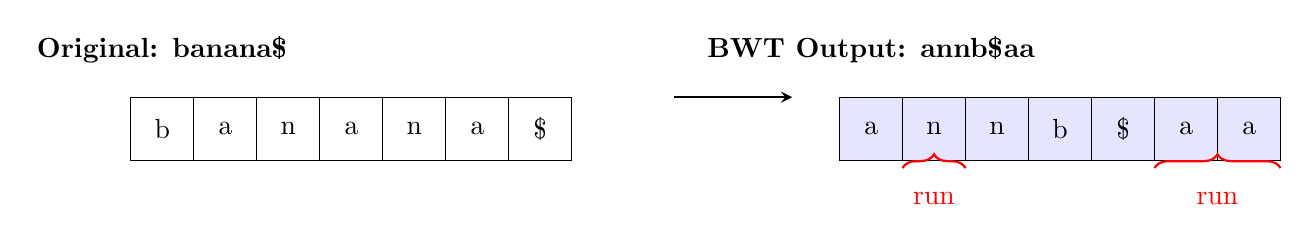
\begin{tikzpicture}[node distance=1cm, auto]
    % Original string
    \node (title1) at (0,1) {\textbf{Original: banana\$}};
    \foreach \char [count=\i from 0] in {b,a,n,a,n,a,\$} {
        \node[draw, minimum width=0.8cm, minimum height=0.8cm] at (\i*0.8,0) {\char};
    }
    
    % Arrow
    \draw[->, thick, >=stealth] (6.5,0.4) -- (8,0.4);
    
    % BWT output
    \node (title2) at (9,1) {\textbf{BWT Output: annb\$aa}};
    \foreach \char [count=\i from 0] in {a,n,n,b,\$,a,a} {
        \node[draw, minimum width=0.8cm, minimum height=0.8cm, fill=blue!10] at (9+\i*0.8,0) {\char};
    }
    
    % Highlight runs
    \draw[red, thick, decorate, decoration={brace, amplitude=5pt}] (9.4,-0.5) -- (10.2,-0.5) node[midway, below, yshift=-5pt] {run};
    \draw[red, thick, decorate, decoration={brace, amplitude=5pt}] (12.6,-0.5) -- (14.2,-0.5) node[midway, below, yshift=-5pt] {run};
\end{tikzpicture}
\end{center}

The BWT output has:
\begin{itemize}
    \item A run of two 'n's (positions 2-3)
    \item A run of two 'a's at the end (positions 6-7)
    \item The original had \emph{no} runs at all!
\end{itemize}

\subsection{Formal Definition of the BWT}

\subsubsection{Cyclic Rotations and Lexicographic Sorting}

Let us formalize what we have done. Given an input string \(S\) of length \(n\) with a unique end-of-string marker \(\$\) that is lexicographically smaller than all other characters:

\begin{definitionbox}[Burrows-Wheeler Transform]
The Burrows-Wheeler Transform of \(S\), denoted \(\text{BWT}(S)\), is computed as:

\begin{enumerate}
    \item Form a matrix \(M\) of size \(n \times n\) where row \(i\) (0-indexed) is the cyclic rotation of \(S\) starting at position \(i\): 
    \[ M[i] = S[i:] + S[:i] \]
    
    \item Sort the rows of \(M\) in lexicographic order (dictionary order, with '\$' < all other characters).
    
    \item Let \(I\) be the index of the row containing the original string \(S\) in the sorted matrix.
    
    \item The BWT output \(L\) is the last column of the sorted matrix: 
    \[ L[j] = M_{\text{sorted}}[j][n-1] \]
    
    \item The transform also outputs \(I\), the index of the original row, which is needed for inversion.
\end{enumerate}

Thus, \(\text{BWT}(S) = (L, I)\).
\end{definitionbox}

In our ``banana\$'' example:
\begin{itemize}
    \item \(L = \text{``annb\$aa''}\)
    \item \(I = 4\) (the original string ``banana\$'' appears at row 5, which is index 4 in 0-based indexing)
\end{itemize}

\subsubsection{The Last Column Construction}

Why do we take the last column? Consider any two rows that are adjacent in the sorted order. They share a common prefix (the longer the prefix, the more similar their contexts). The last characters of these rows are the characters that \emph{precede} these contexts in the original string. When contexts are similar, the preceding characters often come from a limited set, creating runs.

\begin{importantbox}
The BWT is a \emph{reversible} transformation. Given only \(L\) (the last column) and \(I\) (the index of the original row), we can reconstruct the original string \(S\) exactly. This reversibility is what makes the transform useful for compression—we can recover the original data after decompression.
\end{importantbox}

\subsubsection{Properties of the Transform}

The BWT has several remarkable properties:

\begin{enumerate}
    \item \textbf{Reversibility:} The transform is bijective—every input string maps to a unique \((L, I)\) pair, and the mapping is invertible.
    
    \item \textbf{Run Formation:} The output \(L\) tends to contain long runs of identical characters, especially in structured data like text.
    
    \item \textbf{Context Grouping:} Characters that appear in similar contexts in the original string are brought together in the output.
    
    \item \textbf{Structure Revealing:} Higher-order dependencies in the original string become lower-order dependencies in the transformed string.
    
    \item \textbf{Block Structure:} The transform operates on fixed-size blocks (typically 100KB–900KB), allowing a trade-off between compression ratio and memory usage.
\end{enumerate}

\subsection{Inverting the BWT}

The inversion algorithm is where the true cleverness of the BWT reveals itself. Given only \(L\) (the last column) and \(I\) (the index of the original row), we can reconstruct the original string without ever storing the full rotation matrix.

\subsubsection{The First–Last (LF) Mapping}

The key insight is that the first column \(F\) of the sorted rotation matrix can be derived from \(L\) alone:

\begin{enumerate}
    \item \(F\) is simply \(L\) sorted lexicographically.
    \item Why? Because the rows are sorted lexicographically, the first column is just all characters of the original string in sorted order.
\end{enumerate}

In our example:
\begin{itemize}
    \item \(L = [a, n, n, b, \$, a, a]\)
    \item Sorting \(L\) gives: \([\$, a, a, a, b, n, n] = F\)
\end{itemize}

Now we have a crucial observation: For any character in the last column, we can find its corresponding character in the first column through a mapping that preserves the relative order of identical characters.

\begin{definitionbox}[LF-Mapping]
The LF-mapping (Last-to-First mapping) is a function \(\text{LF}(i)\) that returns the row index in the first column that corresponds to the same character occurrence as position \(i\) in the last column.

For a character \(c\) that appears \(k\) times in the string, the \(k\) occurrences appear in the same order in both \(F\) and \(L\). Therefore, if \(L[i]\) is the \(r\)-th occurrence of character \(c\) in \(L\) (counting from 1), then \(\text{LF}(i)\) is the position of the \(r\)-th occurrence of \(c\) in \(F\).
\end{definitionbox}

\subsubsection{Computing the LF-Mapping Correctly}

Let us compute the LF-mapping for our example step by step.

First, determine the rank of each character in \(L\) (the occurrence number):

\begin{center}
\begin{tabular}{c|c|c|c}
\textbf{Index \(i\)} & \textbf{\(L[i]\)} & \textbf{Rank in \(L\)} & \textbf{Explanation} \\
\hline
0 & a & 1 & First 'a' in L \\
1 & n & 1 & First 'n' in L \\
2 & n & 2 & Second 'n' in L \\
3 & b & 1 & First 'b' in L \\
4 & \$ & 1 & First '\$' in L \\
5 & a & 2 & Second 'a' in L \\
6 & a & 3 & Third 'a' in L \\
\end{tabular}
\end{center}

Now, determine the rank of each character in \(F\):

\begin{center}
\begin{tabular}{c|c|c|c}
\textbf{Index \(j\)} & \textbf{\(F[j]\)} & \textbf{Rank in \(F\)} & \textbf{Explanation} \\
\hline
0 & \$ & 1 & First '\$' in F \\
1 & a & 1 & First 'a' in F \\
2 & a & 2 & Second 'a' in F \\
3 & a & 3 & Third 'a' in F \\
4 & b & 1 & First 'b' in F \\
5 & n & 1 & First 'n' in F \\
6 & n & 2 & Second 'n' in F \\
\end{tabular}
\end{center}

The LF-mapping matches each position \(i\) in \(L\) to the position \(j\) in \(F\) that has the same character and the same rank:

\begin{center}
\begin{tabular}{c|c|c|c|c}
\textbf{\(i\)} & \textbf{\(L[i]\)} & \textbf{Rank in \(L\)} & \textbf{Matches in \(F\)} & \textbf{\(LF[i]\)} \\
\hline
0 & a & 1 & First 'a' in F at index 1 & 1 \\
1 & n & 1 & First 'n' in F at index 5 & 5 \\
2 & n & 2 & Second 'n' in F at index 6 & 6 \\
3 & b & 1 & First 'b' in F at index 4 & 4 \\
4 & \$ & 1 & First '\$' in F at index 0 & 0 \\
5 & a & 2 & Second 'a' in F at index 2 & 2 \\
6 & a & 3 & Third 'a' in F at index 3 & 3 \\
\end{tabular}
\end{center}

Thus, the correct LF-mapping array is:
\[ LF = [1, 5, 6, 4, 0, 2, 3] \]

\subsubsection{Reconstruction Algorithm}

With the correct LF-mapping, we can now reconstruct the original string by walking backwards from the known original row:

\begin{algorithm}[H]
\caption{BWT Inversion}
\begin{algorithmic}[1]
\Require \(L[0..n-1]\) (last column), \(I\) (index of original row)
\Ensure Original string \(S\)

\State \(n \gets \text{length}(L)\)
\State Compute \(F \gets \text{sort}(L)\)
\State Build LF-mapping array \(LF[0..n-1]\) as described above
\State Initialize \(S\) as empty string
\State \(row \gets I\)

\For{\(k \gets 0\) to \(n-1\)}
    \State Prepend \(L[row]\) to \(S\) \Comment{Add character to front}
    \State \(row \gets LF[row]\) \Comment{Move to previous row}
\EndFor

\State \Return \(S\)
\end{algorithmic}
\end{algorithm}

\begin{examplebox}[Correct Inversion of ``annb\$aa'' with I=4]
Let us trace through the inversion using our correct LF-mapping:

\(LF = [1, 5, 6, 4, 0, 2, 3]\), \(I = 4\)

We will walk backwards, prepending each character we encounter:

\begin{center}
\begin{tabular}{c|c|c|c}
\textbf{Step} & \textbf{Current Row} & \textbf{Character to Prepend} & \textbf{New Row (\(LF[row]\))} \\
\hline
Start & 4 & & \\
1 & 4 & \(L[4] = \$\) & \(LF[4] = 0\) \\
2 & 0 & \(L[0] = a\) & \(LF[0] = 1\) \\
3 & 1 & \(L[1] = n\) & \(LF[1] = 5\) \\
4 & 5 & \(L[5] = a\) & \(LF[5] = 2\) \\
5 & 2 & \(L[2] = n\) & \(LF[2] = 6\) \\
6 & 6 & \(L[6] = a\) & \(LF[6] = 3\) \\
7 & 3 & \(L[3] = b\) & \(LF[3] = 4\) \\
\end{tabular}
\end{center}

Now, let's track the string being built by prepending each character:

\begin{center}
\begin{tabular}{c|c|c}
\textbf{Step} & \textbf{Character Prepended} & \textbf{Current String \(S\)} \\
\hline
1 & \$ & ``\$'' \\
2 & a & ``a\$'' \\
3 & n & ``na\$'' \\
4 & a & ``ana\$'' \\
5 & n & ``nana\$'' \\
6 & a & ``anana\$'' \\
7 & b & ``banana\$'' \\
\end{tabular}
\end{center}

Perfect! We have successfully reconstructed ``banana\$''. The key was having the correct LF-mapping that preserves the order of identical characters.
\end{examplebox}

\subsubsection{Proof of Correctness (Sketch)}

The inversion algorithm works because of a fundamental property of the sorted rotation matrix:

\begin{theorem}[LF-Mapping Property]
For any row \(i\) in the sorted rotation matrix, the character \(L[i]\) (last column) is the character that precedes \(F[i]\) (first column) in the original string. Moreover, the row \(LF[i]\) in the sorted matrix corresponds to the rotation that starts with \(L[i]\).
\end{theorem}

This creates a chain that cycles through all rows exactly once. Starting from the row containing the original string (index \(I\)) and following the LF-mapping backwards, we visit each row exactly once in reverse cyclic order, allowing us to reconstruct the original string by collecting the last column characters in reverse order.

\subsection{Why BWT Improves Compressibility}

\subsubsection{Run Formation and Structure Revelation}

The BWT's power for compression comes from its tendency to create runs of identical characters. To understand why, consider the following:

\begin{enumerate}
    \item In the sorted rotation matrix, rows with similar prefixes are adjacent.
    \item The last column contains the characters that \emph{precede} these prefixes in the original string.
    \item If the original text has statistical regularities (e.g., 'q' is almost always followed by 'u'), then all rows starting with 'u' will be adjacent, and their last characters will all be 'q' (or characters that commonly precede 'u').
\end{enumerate}

\begin{importantbox}[Important Clarification on Entropy]
It is crucial to understand that the BWT does \textbf{not} reduce the zero-order entropy of the data. In fact, the zero-order entropy of \(L\) equals that of \(S\) because the transform is a permutation of the original characters.

What the BWT achieves is something more subtle: it transforms \textbf{higher-order dependencies} in the original string into \textbf{lower-order dependencies} in the transformed string. After BWT, patterns that were previously spread across the text become localized, making them exploitable by simple zero-order coding methods like Move-To-Front and Run-Length Encoding.

In other words, the BWT rearranges the data so that the \emph{conditional probabilities} that characterize higher-order structure become visible as \emph{empirical frequencies} that zero-order coders can exploit.
\end{importantbox}

\begin{examplebox}[Visualizing the Effect]
Consider English text. The character 'u' frequently follows 'q'. In the original text, these 'u's are scattered. In the BWT output:
\begin{itemize}
    \item All occurrences of 'u' (as first column entries) will be grouped together because rotations starting with 'u' are adjacent in sorted order.
    \item Their corresponding last column entries will be the characters that preceded these 'u's—often 'q'.
    \item Result: A run of 'q's appears in the output, which can be efficiently compressed by RLE.
\end{itemize}
\end{examplebox}

\subsubsection{Connection to Context Modeling}

Recall from Lecture 4 that higher-order Markov models capture dependencies by considering the previous \(k\) characters. The BWT achieves something analogous without explicit probability modeling:

\begin{itemize}
    \item In Lecture 4, we built explicit models: \(P(\text{next symbol} \mid \text{previous } k \text{ symbols})\)
    \item In BWT, sorting rotations groups symbols that share the same context (the following characters)
    \item The result is that conditional probabilities become visible as local patterns in the output
\end{itemize}

This is why BWT can be seen as an \emph{implicit context modeling} transform—it reorganizes data so that context-dependent structure becomes spatially local.

\begin{importantbox}
The BWT doesn't compress; it reveals structure. The actual compression is done by subsequent stages that exploit the local correlations the BWT creates.
\end{importantbox}

\subsection{The Full BWT Compression Pipeline}

A complete BWT-based compressor typically consists of several stages:

\begin{center}
\begin{tikzpicture}[node distance=1.5cm, auto]
    % Nodes
    \node (input) [draw, rectangle] {Original Data};
    \node (bwt) [draw, rectangle, right=of input] {BWT};
    \node (mtf) [draw, rectangle, right=of bwt] {Move-To-Front};
    \node (rle) [draw, rectangle, right=of mtf] {RLE};
    \node (entropy) [draw, rectangle, right=of rle] {Entropy Coding};
    \node (output) [draw, rectangle, right=of entropy] {Compressed Data};
    
    % Arrows
    \draw[->] (input) -- (bwt);
    \draw[->] (bwt) -- (mtf);
    \draw[->] (mtf) -- (rle);
    \draw[->] (rle) -- (entropy);
    \draw[->] (entropy) -- (output);
\end{tikzpicture}
\end{center}

\subsubsection{Move-To-Front (MTF) Encoding}

After the BWT, we have a string with local correlations but not yet in a form optimal for entropy coding. Move-To-Front encoding transforms this string into a sequence of small integers that are highly compressible.

\begin{definitionbox}[Move-To-Front Encoding]
The MTF encoder maintains a list of symbols. For each input symbol:
\begin{enumerate}
    \item Output its current index in the list (0-based)
    \item Move that symbol to the front of the list
\end{enumerate}
\end{definitionbox}

\begin{examplebox}[MTF of BWT Output]
For pedagogical clarity, we use a simplified alphabet containing only the characters that appear in our example: \([a, b, n, \$]\). In practice, MTF operates on the full byte alphabet (0–255), but the principle remains identical.

Apply MTF to ``annb\$aa'' with initial list [a, b, n, \$] (sorted order for predictability):

\begin{center}
\begin{tabular}{c|c|c|c}
\textbf{Input} & \textbf{Current List} & \textbf{Index} & \textbf{Output} \\
\hline
a & [a, b, n, \$] & 0 & 0 \\
  & Move a to front → [a, b, n, \$] (already at front) & & \\
n & [a, b, n, \$] & 2 & 2 \\
  & Move n to front → [n, a, b, \$] & & \\
n & [n, a, b, \$] & 0 & 0 \\
  & Move n to front → [n, a, b, \$] (already at front) & & \\
b & [n, a, b, \$] & 2 & 2 \\
  & Move b to front → [b, n, a, \$] & & \\
\$ & [b, n, a, \$] & 3 & 3 \\
  & Move \$ to front → [\$, b, n, a] & & \\
a & [\$, b, n, a] & 3 & 3 \\
  & Move a to front → [a, \$, b, n] & & \\
a & [a, \$, b, n] & 0 & 0 \\
  & Move a to front → [a, \$, b, n] & & \\
\end{tabular}
\end{center}

MTF output: [0, 2, 0, 2, 3, 3, 0]

Notice how runs of identical symbols in the BWT output become runs of zeros in the MTF output! This is the key to BWT's effectiveness—local structure in the BWT output translates to runs of small numbers after MTF.
\end{examplebox}

\subsubsection{Run-Length Encoding (RLE)}

After MTF, we have a sequence dominated by small numbers, often with long runs of zeros. Run-length encoding compresses these runs efficiently.

\begin{examplebox}[RLE of MTF Output]
MTF output: [0, 2, 0, 2, 3, 3, 0]

After RLE (encoding runs of identical values):
\begin{itemize}
    \item 0 appears alone (position 1) → encode as (0,1)
    \item 2 appears alone → (2,1)
    \item 0 appears alone → (0,1)
    \item 2 appears alone → (2,1)
    \item 3 appears as a run of length 2 → (3,2)
    \item 0 appears alone → (0,1)
\end{itemize}

RLE output: (0,1), (2,1), (0,1), (2,1), (3,2), (0,1)

This representation has even lower entropy than the MTF output.
\end{examplebox}

\subsubsection{Final Entropy Coding (Huffman or Arithmetic)}

The final stage applies statistical coding (Huffman or arithmetic coding) to the RLE output. Because the data now consists of small integers with skewed distributions, entropy coding achieves excellent compression ratios.

\subsection{Efficient Implementation}

\subsubsection{Naive Rotation Matrix: Why It Is Impractical}

The naive BWT implementation described earlier—constructing an \(n \times n\) matrix of rotations—is completely impractical for real data:

\begin{itemize}
    \item For a 1MB file (\(n \approx 10^6\)), storing all rotations would require \(10^{12}\) characters (1TB) of memory!
    \item Even storing indices rather than full strings, we need \(n\) rotations of length \(n\), which is \(O(n^2)\) space.
\end{itemize}

Clearly, we need a more efficient approach.

\subsubsection{Suffix Arrays for Efficient Construction}

The key insight is that we don't need to store all rotations explicitly. For a string with a unique end marker, the cyclic rotations correspond exactly to the suffixes of the string when we consider the end marker as a special character.

\begin{definitionbox}[Suffix Array]
A suffix array for a string \(T\) of length \(n\) is an array of integers \(SA[0..n-1]\) that gives the starting positions of the suffixes of \(T\) in lexicographic order.
\end{definitionbox}

For BWT construction, we only need the suffix array of \(S\$\) (the original string with the unique end marker). The relationship is:

\begin{itemize}
    \item The suffix starting at position \(i\) corresponds to the rotation that begins at position \(i\) in the original string.
    \item The lexicographic order of suffixes is identical to the lexicographic order of rotations because the end marker ensures no suffix is a prefix of another.
\end{itemize}

\begin{algorithm}[H]
\caption{Efficient BWT Construction Using Suffix Arrays}
\begin{algorithmic}[1]
\Require Input string \(S\) of length \(n\) with unique end marker '\$'
\Ensure BWT output \(L[0..n-1]\) and primary index \(I\)

\State \(T \gets S\) \Comment{\(T\) includes the end marker}
\State Build suffix array \(SA\) for \(T\) \Comment{\(O(n \log n)\) or \(O(n)\) time}

\For{\(i \gets 0\) to \(n-1\)}
    \State \(pos \gets SA[i]\)
    \If{\(pos = 0\)}
        \State \(L[i] \gets \$\) \Comment{Last character when suffix starts at beginning}
        \State \(I \gets i\) \Comment{Record position of original string}
    \Else
        \State \(L[i] \gets T[pos-1]\) \Comment{Character before this suffix}
    \EndIf
\EndFor

\State \Return \((L, I)\)
\end{algorithmic}
\end{algorithm}

\subsubsection{Time and Space Complexity}

Modern BWT implementations achieve excellent efficiency:

\begin{itemize}
    \item \textbf{Time Complexity:} \(O(n \log n)\) for sorting-based suffix array construction, or \(O(n)\) for advanced algorithms (SA-IS, DC3)
    \item \textbf{Space Complexity:} \(O(n)\) for the suffix array plus input/output buffers
    \item \textbf{Practical Performance:} \texttt{bzip2} processes data at several MB/s, with block sizes typically 100KB–900KB
\end{itemize}

\begin{importantbox}
The development of practical linear-time suffix array construction algorithms and efficient in-place implementations was crucial for making BWT feasible for real-world compression.
\end{importantbox}

\subsection{Comparison with Lempel--Ziv Methods}

\subsubsection{Local vs. Global Redundancy}

The fundamental difference between LZ77 and BWT lies in how they exploit redundancy:

\begin{center}
\begin{tabularx}{\textwidth}{@{}l X X@{}}
\toprule
\textbf{Aspect} & \textbf{LZ77 (DEFLATE)} & \textbf{BWT (bzip2)} \\
\midrule
Redundancy Type & Local (within sliding window) & Global (across entire block) \\
Detection Method & String matching in window & Sorting all rotations \\
Memory Reference & Explicit (distance, length) & Implicit (context grouping) \\
Adaptivity & Online (streaming) & Block-based \\
\bottomrule
\end{tabularx}
\end{center}

\subsubsection{Compression Ratio vs. Speed Trade-offs}

\begin{center}
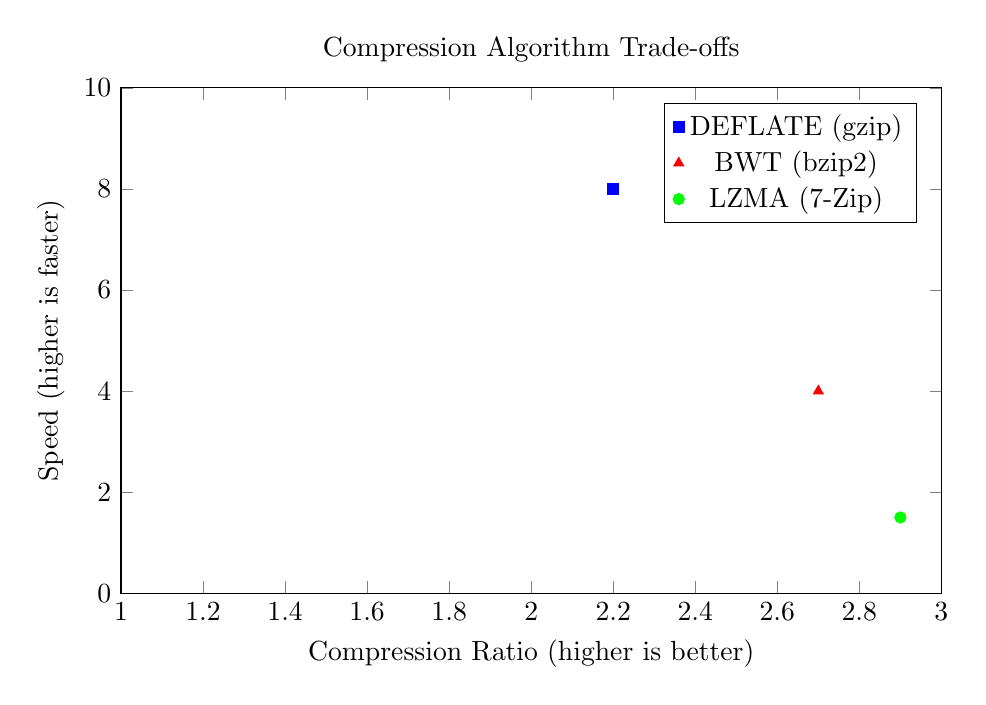
\begin{tikzpicture}
\begin{axis}[
    xlabel={Compression Ratio (higher is better)},
    ylabel={Speed (higher is faster)},
    xmin=1, xmax=3,
    ymin=0, ymax=10,
    width=12cm,
    height=8cm,
    scatter/classes={
        a={mark=square*,blue},
        b={mark=triangle*,red},
        c={mark=*,green}
    },
    legend pos=north east,
    title={Compression Algorithm Trade-offs}
]

% DEFLATE (gzip)
\addplot[scatter,only marks,mark=square*,blue]
    coordinates {(2.2,8)} \closedcycle;
\addlegendentry{DEFLATE (gzip)}

% BWT (bzip2)
\addplot[scatter,only marks,mark=triangle*,red]
    coordinates {(2.7,4)} \closedcycle;
\addlegendentry{BWT (bzip2)}

% LZMA (7-Zip)
\addplot[scatter,only marks,mark=*,green]
    coordinates {(2.9,1.5)} \closedcycle;
\addlegendentry{LZMA (7-Zip)}

\end{axis}
\end{tikzpicture}
\end{center}

\subsection{Case Study: \texttt{bzip2}}

\subsubsection{Architecture Overview}

\texttt{bzip2} is the canonical BWT-based compressor. Its pipeline is:

\begin{enumerate}
    \item \textbf{Run-Length Encoding Prelim:} A preliminary RLE stage to compress repeated characters (simplifies later stages)
    \item \textbf{Burrows-Wheeler Transform:} Applied to blocks (default 900KB)
    \item \textbf{Move-To-Front Transform:} Converts local correlations into runs of zeros
    \item \textbf{Run-Length Encoding:} Compresses runs from MTF
    \item \textbf{Huffman Coding:} Multiple Huffman tables for different parts of the data
\end{enumerate}

\subsubsection{Why BWT Beats DEFLATE on Text}

On natural language text, \texttt{bzip2} typically achieves 15-30\% better compression than \texttt{gzip} because:

\begin{itemize}
    \item Text has global structure (frequent words, common phrases) that spans entire documents
    \item LZ77's window limits miss these long-range dependencies
    \item BWT's global reordering captures these dependencies implicitly
\end{itemize}

\begin{examplebox}[Compression Comparison]
On the Canterbury Corpus (standard compression benchmark):
\begin{itemize}
    \item File: \texttt{alice29.txt} (Alice in Wonderland, 152KB)
    \item \texttt{gzip -9}: 56KB (compression ratio 2.71)
    \item \texttt{bzip2 -9}: 44KB (compression ratio 3.45)
    \item Improvement: 21\% better compression
\end{itemize}
\end{examplebox}

\subsection{Limitations and Modern Extensions}

\subsubsection{Block Size Constraints}

BWT operates on fixed-size blocks. The choice of block size involves trade-offs:

\begin{itemize}
    \item \textbf{Larger blocks:} Better compression (more context), but more memory, slower processing
    \item \textbf{Smaller blocks:} Faster, less memory, but poorer compression
\end{itemize}

\texttt{bzip2} allows block sizes from 100KB to 900KB. Beyond 900KB, compression gains diminish while memory usage grows linearly.

\subsubsection{Memory Usage Considerations}

BWT requires:
\begin{itemize}
    \item \(O(n)\) memory for the suffix array (4-8 bytes per character)
    \item Additional memory for MTF and RLE stages
    \item For 900KB blocks, \texttt{bzip2} uses about 7MB of RAM—modest by modern standards but significant for embedded systems
\end{itemize}

\subsubsection{When BWT May Not Improve Compression}

While BWT is reversible and theoretically cannot reduce compressibility, in practice several factors can lead to worse compression than simpler methods:

\begin{itemize}
    \item \textbf{Block overhead:} The transform operates on fixed-size blocks. Very small blocks (< 1KB) may have overhead that outweighs any compression benefit.
    
    \item \textbf{Primary index storage:} The index \(I\) must be stored with each block, adding a small constant overhead.
    
    \item \textbf{MTF inefficiency on random data:} If the input has no structure, sorting creates no useful patterns, and MTF may actually increase the entropy by spreading out values.
    
    \item \textbf{Algorithmic overhead:} The multi-stage pipeline (BWT + MTF + RLE + entropy coding) adds computational cost that may not be justified for data that compresses well with simpler methods.
\end{itemize}

For these reasons, BWT-based compressors like \texttt{bzip2} excel on structured data like text but may be outperformed by simpler LZ77 variants on binary data or already-compressed files.

\subsubsection{Relation to FM-Index and Text Indexing}

The BWT's impact extends far beyond compression. In 2000, Paolo Ferragina and Giovanni Manzini introduced the FM-index (Full-text index in Minute space), which uses the BWT to create a compressed data structure that supports:

\begin{itemize}
    \item \textbf{Counting queries:} Find the number of occurrences of a pattern \(P\) in \(O(|P|)\) time, regardless of the text size.
    \item \textbf{Locating queries:} Find the positions of matches in \(O(|P| + \text{occ} \cdot \log^\epsilon n)\) time, where occ is the number of occurrences and the log factor depends on sampling rates.
    \item \textbf{Extract queries:} Retrieve arbitrary substrings of the original text without full decompression.
\end{itemize}

The FM-index revolutionized bioinformatics:
\begin{itemize}
    \item \textbf{Bowtie and BWA:} DNA sequence aligners used in countless genomics projects, aligning millions of short reads against reference genomes.
    \item \textbf{Pattern matching in compressed data:} Search without full decompression, enabling efficient querying of large genomic databases.
    \item \textbf{Compressed suffix arrays:} Building block for many string algorithms that operate directly on compressed representations.
\end{itemize}

\begin{importantbox}
The BWT demonstrates a profound principle: compression and indexing are two sides of the same coin. A good compressed representation often enables fast search directly on the compressed data, with time complexity that depends only on pattern size, not on text size.
\end{importantbox}

\subsection{Summary and Key Insights}

\subsubsection{The Transform-Then-Compress Principle}

The BWT embodies a powerful design philosophy:

\begin{enumerate}
    \item \textbf{Separate concerns:} First transform the data to reveal its structure, then compress the transformed representation
    \item \textbf{Reversibility is key:} The transform must be exactly invertible
    \item \textbf{Structure exploitation:} Different transforms reveal different kinds of structure
\end{enumerate}

\subsubsection{When to Use BWT-Based Compression}

\begin{center}
\begin{tabularx}{\textwidth}{@{}l X X@{}}
\toprule
\textbf{Scenario} & \textbf{Recommendation} & \textbf{Rationale} \\
\midrule
Text files, source code & BWT (bzip2) & Global repetition matters \\
Web content (HTTP) & DEFLATE/gzip & Streaming, compatibility \\
Archival storage & LZMA, Zstandard & Maximum compression \\
Real-time systems & LZ77 variants & Low latency, streaming \\
Embedded systems & Custom/simple RLE & Memory constraints \\
DNA sequences & BWT-based + FM-index & Search+compress combined \\
\bottomrule
\end{tabularx}
\end{center}

\subsubsection{Beyond Compression: The FM-Index Revolution}

The BWT's legacy extends far beyond file compression:

\begin{itemize}
    \item \textbf{Compressed data structures:} Store data in compressed form while supporting queries
    \item \textbf{Bioinformatics:} Billions of DNA reads aligned daily using BWT-based tools
    \item \textbf{Information retrieval:} Compressed full-text search engines
    \item \textbf{Theory:} Deep connections between sorting, compression, and indexing
\end{itemize}

\subsection{Hands-On Exercises}

\begin{exercisebox}
Apply the Burrows-Wheeler Transform to the string ``mississippi\$'' by hand. Show:
\begin{enumerate}
    \item All cyclic rotations
    \item The sorted rotations
    \item The BWT output L and primary index I
    \item Identify any runs in the output
\end{enumerate}
\end{exercisebox}

\begin{exercisebox}
Implement a simple BWT encoder in Python:
\begin{lstlisting}[language=Python]
def bwt_encode(s):
    """Return BWT(s) and primary index."""
    # Add end marker
    s = s + '$'
    # Generate rotations (hint: use list comprehension)
    # Sort rotations
    # Extract last column and find original row
    # Return (L, I)
    pass
\end{lstlisting}
Test your implementation on ``banana'' and ``mississippi''.
\end{exercisebox}

\begin{exercisebox}
Compare compression performance on a text file:
\begin{enumerate}
    \item Find a text file > 1MB (e.g., a book from Project Gutenberg)
    \item Compress with \texttt{gzip -9} and \texttt{bzip2 -9}
    \item Compare sizes and compression times
    \item Use \texttt{time} command to measure speed
    \item Explain the results in terms of the algorithms' characteristics
\end{enumerate}
\end{exercisebox}

\begin{exercisebox}
Challenge: Why does BWT perform poorly on random data? Connect your answer to:
\begin{enumerate}
    \item The sorting process in BWT
    \item The subsequent MTF and RLE stages
    \item The concept of structure versus randomness
\end{enumerate}
\end{exercisebox}

\begin{exercisebox}
Research question: The FM-index enables substring search on BWT-compressed data. Explain:
\begin{enumerate}
    \item How the LF-mapping enables backward search
    \item Why counting queries are \(O(|P|)\) time
    \item Applications in bioinformatics (BWA, Bowtie)
\end{enumerate}
\end{exercisebox}

\begin{exercisebox}
Compare the three compression paradigms we've studied:
\begin{center}
\begin{tabularx}{\textwidth}{@{}l X X X@{}}
\toprule
\textbf{Aspect} & \textbf{Statistical} & \textbf{Dictionary} & \textbf{Transform} \\
\midrule
Core idea & Model probabilities & Find repetitions & Reorganize data \\
Example & Huffman, Arithmetic & LZ77, LZ78, DEFLATE & BWT, bzip2 \\
Strengths & Optimal for known model & Fast, adaptive & Global structure \\
Weaknesses & Needs good model & Limited window & Block-based, slower \\
Best for & Well-characterized sources & General purpose & Text, structured data \\
\bottomrule
\end{tabularx}
\end{center}
Fill in this table based on Lectures 1-7.
\end{exercisebox}

\subsection{Looking Forward}

The Burrows-Wheeler Transform concludes our exploration of lossless compression paradigms. In subsequent courses, you may encounter:

\begin{itemize}
    \item \textbf{Transform coding for lossy compression:} DCT in JPEG, wavelets in JPEG2000
    \item \textbf{Context mixing:} PAQ and its descendants (top-tier compression)
    \item \textbf{Asymmetric numeral systems (ANS):} Modern entropy coding used in Facebook's Zstandard
    \item \textbf{Learned compression:} Using machine learning to predict and compress
\end{itemize}

The principles you've learned—entropy as a fundamental limit, the value of modeling, the power of transforms, the trade-offs between speed and ratio—will serve you well in all these advanced topics.

\begin{importantbox}[Key Takeaway]
The Burrows-Wheeler Transform teaches us that sometimes the best way to solve a problem is to transform it into a different problem. By reordering data to reveal its inherent structure, we make the subsequent compression task dramatically easier—a lesson that applies far beyond data compression.
\end{importantbox}
\end{document}
